%% implementation
%!TEX root = ../Project.tex

\section{Implementation}

\subsection{Overview}

\begin{figure}[htbp]
	\centering
		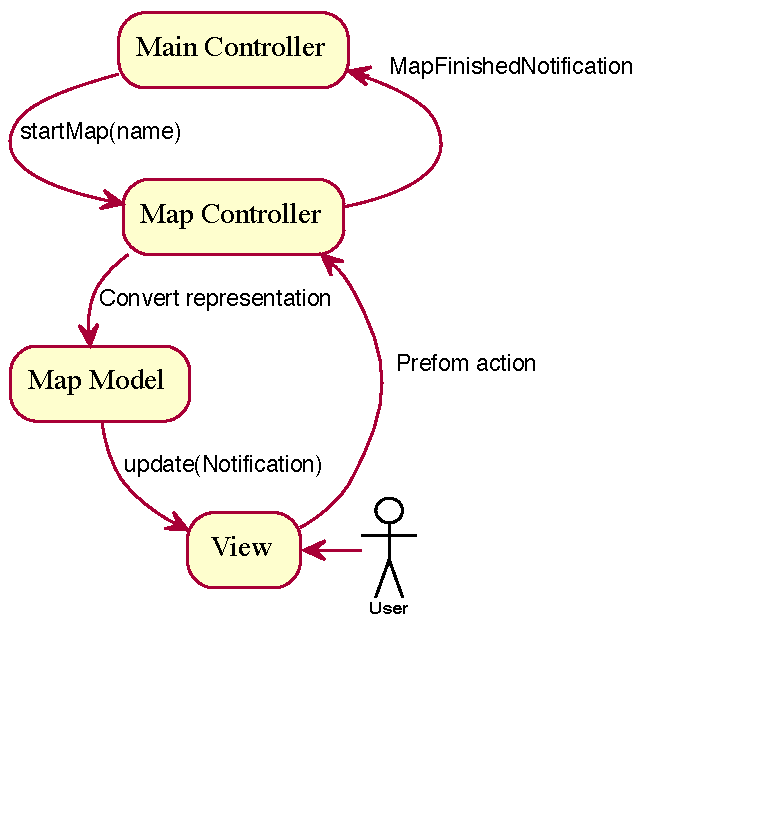
\includegraphics{figures/engine_exported.pdf}
	\caption{Overview of the implementation.}
	\label{fig:overview_engine}
\end{figure}

The system is structured using MVC for the overall architecture as well as  using the Observer Pattern, as shown above.
%TODO explain   Observer Patten somewhere

The \texttt{MainController} handles the overall logic, including the game progression. 
Although the objectives only require an isometric  map view, the implementation was designed to be more general,  hence a \emph{separate} controller for each \texttt{stage} of the game is used. When the \texttt{stage} is finished  (e.g. when a map has been completed) the controller notifies the \texttt{MainController}, which decides what to do next.   

The advantage of this architecture is that it is extendable hence, other \texttt{stages} such as an overworld map or a title screen could be easily added.


The observable components (i.e. the view and the map controller) communicate using \texttt{notification} objects which encapsulate any relevant information. For example, the \texttt{model} sends a \texttt{UnitMovedNotification} when the computer controlled opponent moves one of their units. This notification includes a reference to the unit moved as well as the path it took to get there. The information is used by the GUI to display an animation of the unit moving to the user.

\clearpage
\subsection{Data Format}
\label{sub:data_format}

The schema for the data format was only slightly changed for the reason stated in section \ref{ssub:intercompatibility}. To parse and serialise the xml the \texttt{Xstream} Java library was used\cite{xstream}.
 
XStream is an open source library used to serialise Java objects to and from XML. One of it's major benefits is that it abstracts over the parsing and serialisation and allows the user to focus on what the data should be used for. 

XStream achieves this through the use of Java annotations\footnote{A special form of syntactic metadata that can be added to the source of a Java file, with the notable feature of being retained in the compiled class files.}, as shown in the below example\footnote{Getter, Setters and trivial constructor omitted.}.

\begin{lstlisting}[caption=Example of class that is serialisable with XStream, label=lst:SavedTile, language=java] %Java
	
@XStreamAlias("tile")
public class SavedTile {
	protected final String type;
	protected final int height; 
	protected int startingHeight;
	
	@XStreamAsAttribute
	protected final int x;
	@XStreamAsAttribute
	protected final int y;

	protected Orientation orientation;
	protected String leftWall, rightWall;
	
	private Object readResolve() {
		if (orientation == null)  
			orientation = Orientation.TO_EAST;
		if (startingHeight == 0 && height != 0) startingHeight = height;
		return this;
	}}
\end{lstlisting}

As shown above, no extra logic apart from the annotations is needed for serialisation.  Another benefit of XStream is that it allows setting default values for the fields. This allows the user to omit redundant tags, as shown in the xml where most of the tags have been omitted.
\begin{lst:tile}[caption=Serialised form of the above class. ]
<tile x="0" y="0">
	<type>grass</type>
	<height>1</height>
</tile>
\end{lst:tile}

\subsubsection{Resources}

All resources that are loaded are \texttt{Identifiable}, that is they have a unique id.  There are two main advantages to using this scheme. The first is that it allows cacheing of resources which means that there is only a single instance for each resource (such as weapons and images). This is especially important for the images to reduce the memory requirements as well as the load times.

The other advantage is that I could use the same framework for loading and saving all the resources, hence saving development time as well as reducing code duplication. 

A detail description of the structure and  required resource of a project is in the appendix \ref{sec:project_structure___specification}.

\subsubsection{Sprite Sheets}
\label{ssub:sprite_sheets}


A sprite sheet is a collection of images combined together. The advantage of this is that a single image is loaded, which reduces loading times. It also makes it easier to cache images, since a \emph{subimage} can be efficiently created\footnote{using the Java method \texttt{BufferedImage.getSubimage}}. A \texttt{subimage} shares the same image data as the original so it is an ideal way for each tile to have access to it's images\cite{bufferedImage}.    

\begin{figure}[htbp]
	\centering
		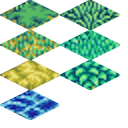
\includegraphics{figures/tileset.png}
	\caption{A 128\*128 sprite sheet containing a tileset for a map}
	\label{fig:figures_tileset}
\end{figure}

Sprite sheets make maps more reusable, since the tileset can be changed without any consequences\footnote{As long as the new tileset has the same number of images or the \texttt{tilemapping} has extra entries for missing images.}.  

I created a sprite sheet editor to allow the user to easily edit the tilesets. Using sprite sheets allows abstracting over the file system, hence increasing the usability of the system. The editor was reused for editing other images such as the character images and it can even be used independently.

\clearpage
\subsection{Engine Development}
\label{sub:engine_development_and_testing}
\subsubsection{Map}
\label{ssub:maps}


The \texttt{Map} class handles the overall logic and game flow.   The main components are:
\begin{itemize}
\item The tiles for the maps. Each tile includes height information as well as the tile's location, as shown in listing \ref{lst:SavedTile}.

\item The enemy units.     

\item The \texttt{TileMapping} which specify what images to use in addition to \emph{how} the tile is drawn. 

\item  The \texttt{conditions} of the maps. These include winning conditions (such as ``Defeat All Enemy Units'',  the placement of player's units and a \texttt{turnComparator} which decides how the turn ordering works.  

\item  The \texttt{events}. These include the dialog which displays parts of the story at the start and end of each battle. 
\end{itemize}

The other major responsibly of the map is to send notifications to the view.  

\subsubsection{Units}
\label{ssub:units}
A \texttt{Unit} has a set of attributes whose values can be specified by the user. A unit is the abstract representation and is used for serialisation.  A \texttt{MapUnit} extends the unit's sets of attributes with extra information such as the location and the current hit points.

A unit has a  specified weapon (as discussed in section \ref{sub:weapons___skills}).  A weapon has an \emph{attack range} which specified how the unit attacks.  As an example, consider a spear which attacks all units in a specified direction and a bow which attack a single faraway target. A unit with the same attributes would play very differently with either of these examples since a spear can only be used in melee combat, whereas a bow can only be used from a distance.

A unit has a set of skills (as descried in section \ref{sub:weapons___skills}). The main difference, apart from the possibility of having \emph{multiple} skills, is the concept of an \texttt{attack area}.  The \emph{attack area} is the tiles that are affected by the skill, which includes \emph{both} friendly and enemy units. A skill can either include the caster in the area or explicitly exclude the caster, which gives the user more flexibility.

While default implementation of skills and weapons are provided, the advance user can create their user using the extension mechanism of the data format (see section \ref{sub:data_format_extension_mechanism}).

\begin{figure}[htbp]
	\centering
 		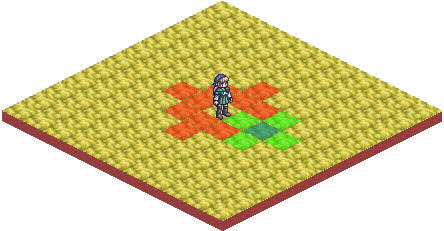
\includegraphics[scale=0.5]{figures/skill.png}
	\caption{An example of a Skill. The red squares are the \emph{attack range}, the green the \emph{attack area}}
	\label{fig:figures_engine_Skills}
\end{figure}

Units can ``level up'' which means the attributes  of the unit increase.  Levelling up can also affect how quickly the unit can get their next turn. levelling up is defined in the battle system as discussed in section \ref{ssub:battle_system}.

When a map has been won all of player's defeated unit's get revived, this is to ensure the next map is completable, and to make the game easier. 

The state machine for the units as described in section \ref{ssub:unit} is implemented using Java \texttt{enums}\footnote{In the class \texttt{view.map.UnitState}}. Java enums differs from a traditional enum in that they can have methods (which are inherently static) and fields.  The advantage of using enums is that they are singleton\footnote{meaning that there is only a single instance of each enum}.  This simplifies the logic, since each enum can return another enum to signal a change of state.

\subsubsection{Movement and Path Finding}

To find the movement range of a unit, Dijkstra's algorithm was used. Dijkstra's algorithm finds the shortest path from a tile to every other tile. This is expensive of course as the maps can be large, so as an improvement I only searched \emph{locally}. Since a unit can move at most \emph{n} squares in any direction, (\emph{n} being the number of tiles the unit is allowed to move) there is no point checking any tile which is more then \emph{n} tiles away.  Searching \emph{locally} means not finding the paths to any \texttt{tile} which is more then \texttt{n} squares are away.

The path is then used to display \emph{animated} unit movement to the user.  This required keeping track of the \emph{direction} in the movement algorithms. 

\def\astar{A$^{\star}$ }

Other algorithms such as \astar (which is generally an improvement on Dijkstra) was considered for finding the shortest path between two tiles. \astar was rejected since it does not provide much improvement since the paths to \emph{every} tile in range are needed. Since the paths were cached, the difference would be negligible and hence it was not worth the time implementing and testing it.

\subsubsection{AI Behaviour}
Each AI unit has a \emph{Behaviour} which specifies how the unit acts and which of the opposing player's units to target.  The engine provides a default implementation which tries to get as close as possible to the target while attacking any of the player's units that happen to be in range on the way.  The targets the engine provides by default include attacking the player's unit that has the lowest hit points and attacking the unit with the highest strength. Like other parts of the engine, a user can user can provide their own behaviour to further customise the game by linking their classes.

\subsubsection{Turn Ordering}
The engine provides dynamic unit ordering.  This allows the ordering to change based on a unit's attributes or actions.  The default implementation allows the unit with the highest \texttt{speed} to move first.  To make the ordering more interesting, it also takes account of the unit's action when deciding which is the next unit to move. For example, if the unit does not move (i.e. uses \texttt{wait}) they get their next turn quicker. As with other parts of the engine the user can use their own classes to further customise the unit ordering.

\subsubsection{Battle System}
\label{ssub:battle_system}

The battle system controls how units interact with each other.  It specifies how damage is calculated as well as any other effects resulting from an action. The engine provides a default implementation where 
\begin{itemize}
	\item The damage dealt by a weapon is calculated by adding the weapon's power to the unit's strength and subtracting the opponent's defence. The least damage a weapon can do is zero, i.e. negative damage is not allowed.
	\item The damage created by a skill is independent of the unit's attributes.
\end{itemize}

The damage caused by a weapon is also affected by the difference in height of the attacker's tile and the target's tile. Attacking from a higher height gives a bonus whereas attacking from below reduces the attack.


The battle system also defines how units ``level up''. The default implementation ``levels up'' a unit when they gain 100 experience points. The unit gains experience points by performing actions. Each action gives a different amount of experience points ranging from none from using \texttt{wait} to 60 (before any modifiers are applied).

The amount of experience gained is dependent on the levels of the attacker and the target. Attacking a higher level unit gives a bonus whereas attacking a lower level unit reduces the amount of experience points gained.

\subsubsection{Conditions}
\label{ssub:events}

A map has a win condition which can be specified by the user.  The engine provides two default implementations, defeat all enemy units and defeat a specific unit.  The user can, of course, provide their own conditions which can be basically anything e.g. move to a specific tile. 

\subsubsection{Dialog}
\label{ssub:dialog}
The engine supports displaying dialog to the user at the start and end of a battle. 

\begin{figure}[htbp]
	\centering
		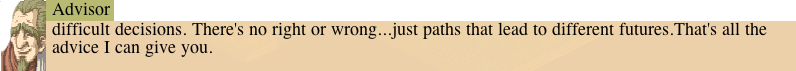
\includegraphics[width=6.3in]{figures/dialog2.png}
	\caption{A example of a dialog}
	\label{fig:figures_dialog2}
\end{figure}

One of the major features is that the engine handles line wrapping and pagination of the text, which is in contrast to many earlier games. This allows the user to focus on writing the plot of the game rather than on fitting the text into the dialog box. 

Optionally, a speaker can be specified for the dialog, this can be used to have a conversation between characters on a map to make the dialog more interactive. 

The editor, as discussed in section \ref{ssub:dialog_editing}, supports editing of the dialog. It has the notable features of allowing the user to visually reorder parts of the dialog. It also supports   importing and exporting the dialog as a text file.  This allows the user to write the script of the game independently in whatever application they prefer. 


\subsection{Saving and Loading}
The engine supports Saving and Loading at any point during the game. The only possible downside  for the user is that when the saved data is loaded, the game continues from the \emph{beginning} of the map which was lasted played. 

The reason for this limitation is to keep the save format small and easy to load. Using this method means the only details that need to be saved are the maps left to be played and the unit's attributes (which can change since units can ``level up''). 

The other limitation is that there is only one save file. This is not a big limitation since the  save file is stored in the user's home directory, meaning each user would have their own save file.

\subsection{Inter-compatibility}
\label{ssub:intercompatibility}
As discussed previously the maps use xml as their data format, one of the advantages of this is that it required very little change to the data format to have incompatibility with Oleksandr Stasyk's  Terrain Generator's output format.  The Terrain generator uses various algorithms to produce a sensible looking map. Users can use these maps as a starting point for their own creation, hence this lowers the time and effort to design a map.

The terrain generator is called by the editor on behalf of the user with appropriate settings\footnote{In the form of a YAML configuration file \texttt{bundle/config.yaml}} saving the user from having to configure the many options available in the terrain generator (since the terrain generator is a command line application).

\subsection{Map Rendering}
\label{ssub:map_rendering}

The GUI uses isometric viewpoint to display the map. 
\begin{figure}[htbp]
	\centering
		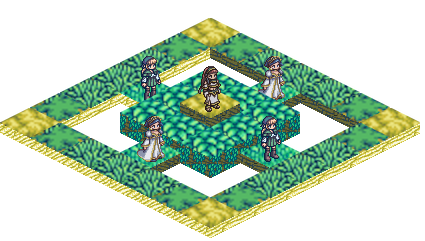
\includegraphics[height=2.8in]{figures/imp-map.png}
	\caption{An isometric map which shows the features of the renderers including height, empty tiles, wall textures and unit placement}
	\label{fig:figures_imp-map}
\end{figure}

The map is composed of isometric tiles which have the following features:

\begin{itemize}[topsep=0mm,noitemsep ]
	\item  The height is \emph{exactly} half the tile's width.
	\item  To create the tile, a square tile is rotated by 45$^{\circ}$ then the height is halved\footnote{A script to do this for the user is provided see \lstinline!scripts/create_isometric_tiles/create_iso_tiles.sh! for details}.
\end{itemize}

One the major features of the map render is how the height is specified.  Instead of using a bunch of careful constructed tiles to simulate height, each tile has a specified height which the renderer uses to draw the tile with appropriate height. 

\subsubsection{Drawing Algorithm}
The algorithm for drawing tiles is firstly the top of the tile is drawn, then the walls are drawn. It is quite general since it supports tiles which can slant in any direction, as shown in figure \ref{fig:mtile2} where the tile is slanting to the north, as well as zooming and arbitrary height \footnote{A simulation of the equations was made first and is in \texttt{other/IsomerticRendering.gcx} (Mac Only).}. 

\def\tileSize{3in}
\begin{figure}[h!tbp]
	\begin{center}
	\subfigure[A Tile with a height(start and end) of 2]{
		\label{fig:mtile1} 
\includegraphics[width=\tileSize]{figures/tile1.png}} 
	\subfigure[A Tile with a start height 1 and an end height of 2 with the walls in green and red]{
		\label{fig:mtile2} 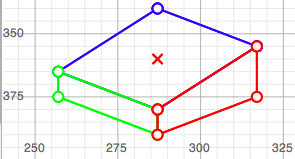
\includegraphics[width=\tileSize]{figures/tile3.png}} 
	\caption{The above figure shows normal and slanted tiles, The red X is the start point for drawing}
	\label{fig:mtile0}
	\end{center}
\end{figure}

Mathematically the set of points used to draw tile are as follows:
\begin{equation}
\; \left[ \begin{array}{c} x \\ y \end{array} \right]=\left\{ \left[ \begin{array}{c} tx \\ ty-h2 \end{array} \right],\left[ \begin{array}{c} tx+\frac{hoz}{2} \\ ty-h2+\frac{vet}{2} \end{array} \right],\left[ \begin{array}{c} tx \\ ty-h1+vet \end{array} \right],\left[ \begin{array}{c} tx-\frac{hoz}{2} \\ ty-h1+\frac{vet}{2} \end{array} \right] \right\}
\end{equation}

\begin{equation}
\; \left[ \begin{array}{c} x \\ y \end{array} \right]=\left\{ \left[ \begin{array}{c} tx \\ ty-h2 \end{array} \right],\left[ \begin{array}{c} tx+\frac{hoz}{2} \\ ty-h2+\frac{vet}{2} \end{array} \right],\left[ \begin{array}{c} tx \\ ty-h1+vet \end{array} \right],\left[ \begin{array}{c} tx-\frac{hoz}{2} \\ ty-h1+\frac{vet}{2} \end{array} \right]\right\}
\end{equation}

\begin{equation}
\hspace{-2.5cm} \left[ \begin{array}{c} x \\ y \end{array} \right]=\left\{ \left[ \begin{array}{c} tx \\ ty-h1+vet \end{array} \right],\left[ \begin{array}{c} tx-\frac{hoz}{2} \\ ty-h1+\frac{vet}{2} \end{array} \right],\left[ \begin{array}{c} tx-\frac{hoz}{2} \\ ty+\frac{vet}{2} \end{array} \right],\left[ \begin{array}{c} tx \\ ty+vet \end{array} \right] \right\}
\end{equation}

\begin{align*}
	tx,\; ty   &\;\; \textrm{is the starting point (shown as an red X in the above figure)}\\
	vet,\; hoz &\;\; \textrm{is the height and width of the tile adjusted for  the zoom and pitch}\\
	h1,\; h2   &\;\; \textrm{are the differences in the start height and end height and vice verse}
\end{align*}

where equation 1 is for the top of the tile, equation 2 for the left wall and equation 3 for the right wall. 

The equation converted to Java easily since the \texttt{Graphic} class has the methods  \texttt{drawPolygon} which draw a polygon using set of points conveniently in the same form as the equations.

%TODO
\subsubsection{Images and Texture Mapping}
The top of tile can be texture mapped or be drawn directly from an image.  Texture mapping repeats a small image across the tile. This is the simpler method for the user since they only have to provide a small texture image, but they lose control over where exactly the image is drawn.  Texture mapping is also required for slanted tiles since there are too many variations to provide images for.

The user also has the option of using an image which is drawn directly. To do this they would have to provide their own isometric tile\footnote{There are scripts to help the user though}. This method allows more control on what is drawn.  

Walls like slanted tiles are always texture mapped since there are to many variations to provide images for. 

\subsubsection{Units}
Each image has at minimum \emph{four} images associated with it, one for each direction (east, west, north, south). These are used to show which way the unit is facing. The unit can also have an animation associated with each direction,to make unit movement more interactive.  The unit can optionally have a portrait which, if available, would be used for their dialog

\subsubsection{Reusability}
Since the map renderer is not dependant on the main GUI, it could be reused in many different places in the editor. 

\subsection{Map Rotation}
The map renderer supports four different rotations which the user can choose from. This is implemented \emph{not} by actually rotating the map (since this would be expensive) but by changing the draw order. By default (0,0) is on the top left of the map. Rotation merely changes the location of (0,0). This means that none of the tile have changed so all the cached calculations can be kept.  Rotating the map can be used by the user to see units that are hidden or obstructed by tiles. 

\subsection{User Interface}
\subsubsection{Controls}
The main control scheme for the GUI is the keyboard, but the user can perform nearly every action using the mouse. All the elements were designed to work equally well with the mouse and keyboard. This means for example that the tiles and units are clickable, (which result in the tile/unit being selected when clicked).  

\subsubsection{Menus}

The GUI uses a menu system to handle the unit's actions. The menu is quite general since it will resize to the longest item in the menu.  It also supports nested menus which are used when the user chooses to use a skill. The menu is controllable using the keyboard arrows keys, but the user can also click an item directly to select it.


\subsubsection{Other Features}
The GUI supports other features to improve the user experience these include:

\begin{itemize}
	\item Zoom in/out which lets the user see more detail. 
	\item Changing the \texttt{pitch} of the map (increasing the pitch flattens the map which allows the user to easily see obstructed units).
	\item A \texttt{log} which can be used to see which actions have taken place. This is useful to find out what the enemy has done if the user misses it the first time.
	\item The key mapping is displayed to the user on startup.
	\item The GUI automatically scrolls to the enemy unit's location if they are out of range when it is their turn.
	\item The unit information shows the unit's attributes including the current hit points. They are displayed in a different colour for opposing units to easily distinguish them. 
\end{itemize}


\subsection{Editor Development}

\subsubsection{Overview}
\label{ssub:overview}

The editor allows the user to customise nearly all aspects of the engine.  Notable features include visual map making as well as exporting the created game as a completely self contained application with \emph{no} external dependencies apart from a recent version of Java\footnote{specify Java 6+}. 

The editor uses a tabbed interface, the benefit is that it shows the users what's available in the editor. Each tab shares the same overall structure for two reasons, namely to keep all aspects of the editor consistent, hence making it easer it to use. The second reason is that most of the code can be reused for each tab, saving development time. 

In each tab the current resources created are listed on the left as shown in figure \ref{fig:figures_editor_Units}. The user can click on any of the resources to customise them. At the bottom of the list are two buttons: the left button (--) removes the selected resource, whereas the right button (+) adds a new resource. Since it is likely the user would create simpler resources (e.g  a weapon of the same type differing only in Strength), any newly created resource takes on the characteristics of the last selected item.

\begin{figure}[htbp]
	\centering
		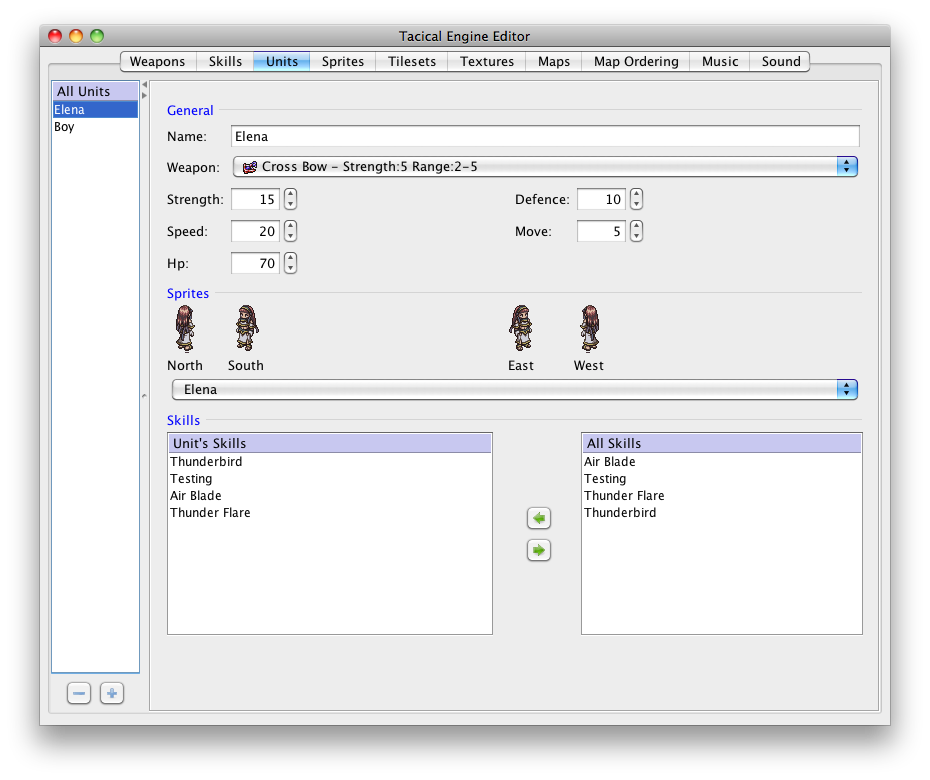
\includegraphics[width=\textwidth]{figures/editor/Units.png}
	\caption{Unit Editor}
	\label{fig:figures_editor_Units}
\end{figure}

To prevent errors and increase usability,  \texttt{JSpinner} was used whenever numeric input was needed. \texttt{JSpinner} also allows a minimum and maximum range to be specified,  the component will then reject any input which is not in range.

Each of the tabs can only edit their own data but they can \emph{read} data from other tabs, as shown above where the weapons and skills are received. One of the advantages is the data is always consistent. This was made a lot simpler since the user can only edit one set of resources at a time.

Since the tabs only expose their resources (instead of handling I/O as well),  this means that the tabs can be reused e.g. (Sprite, Tilesets and textures share nearly all their code).

\subsubsection{Weapons \& Skills}

The editor supports customising of the weapons and skills as shown. 

\def\editor{0.237}
\begin{figure}[htbp]
	\begin{center}
	\subfigure[Weapons Panel]{
		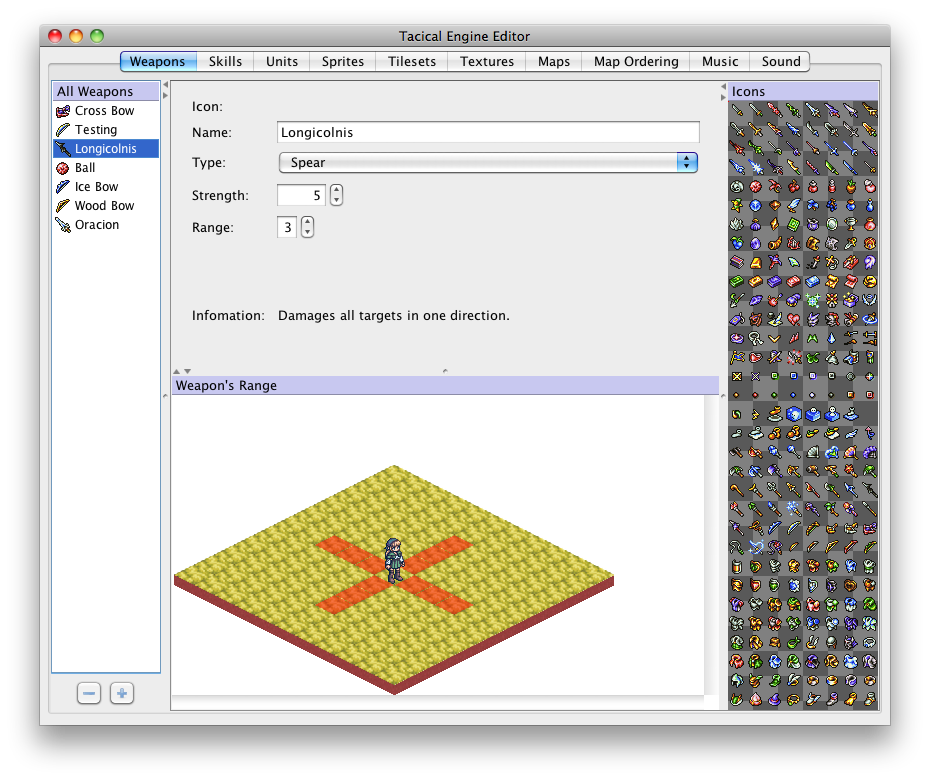
\includegraphics[scale=\editor]{figures/editor/Weapons.png}}
	\subfigure[Skill Panel]{
			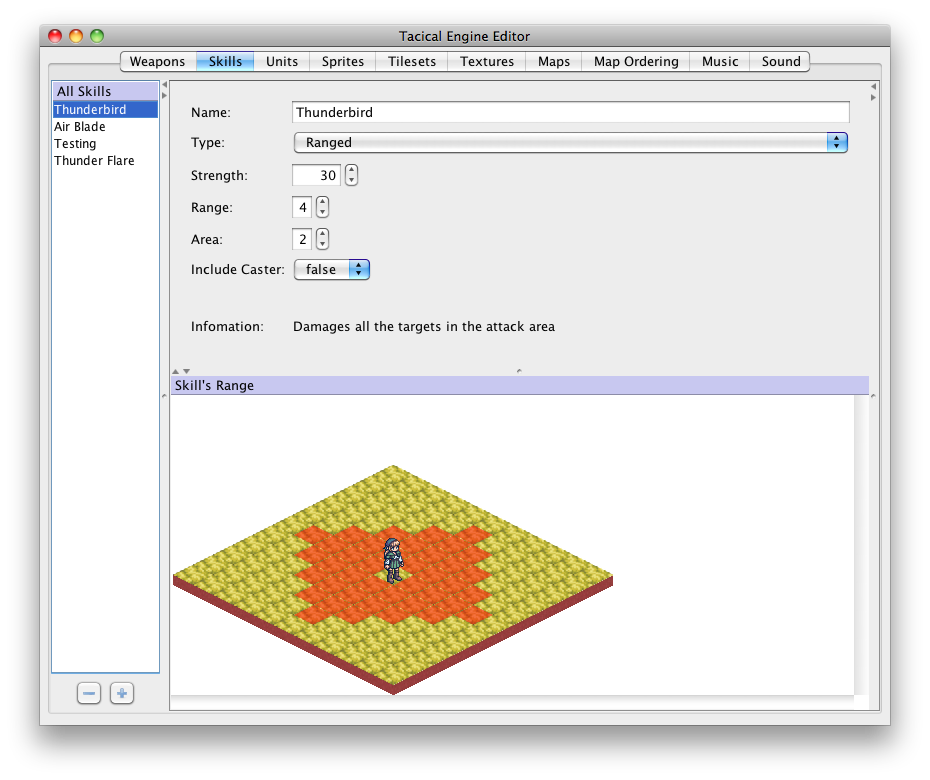
\includegraphics[scale=\editor]{figures/editor/Skills.png}}
	\end{center}
	\label{fig:editor2}
\end{figure}

The editor shows visually what the attack range looks like. This is updated whenever the user makes any change to the resource.  This required very little extra code since the map renderer was general enough to be easily embedded. 

\subsubsection{Unit Editor}
\label{ssub:unit_editors}
The unit allows the user to edit all of the attributes of the units. These include the skills and weapon as well as the images of unit, as shown in figure \ref{fig:figures_editor_Units}. 


\subsubsection{Sprite Sheet Editor}
A sprite sheet editor is used for many of the tabs including the unit's images, textures and tileset.
\begin{figure}[htbp]
	\centering
		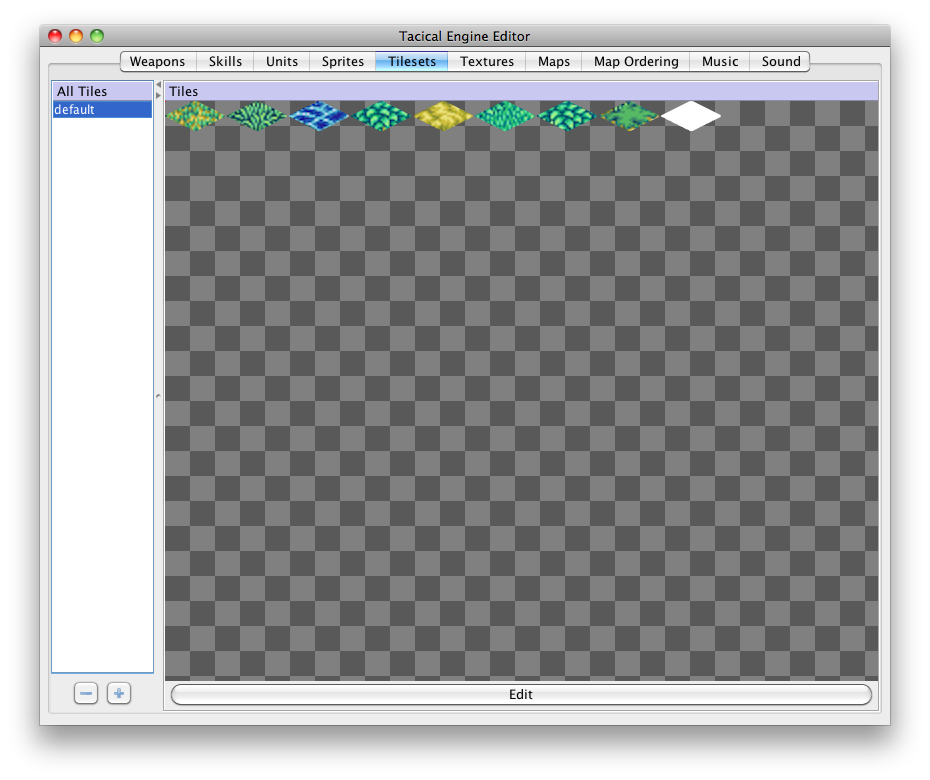
\includegraphics[width=0.75\textwidth]{figures/editor/tileset_edit.png}
	\caption{A sprite sheet  editor for the tiles}
	\label{fig:figures_editor_tileset_edit}
\end{figure}

\subsubsection{Music Editor}
\label{ssub:music_editor}

\begin{figure}[htb]
	\centering
		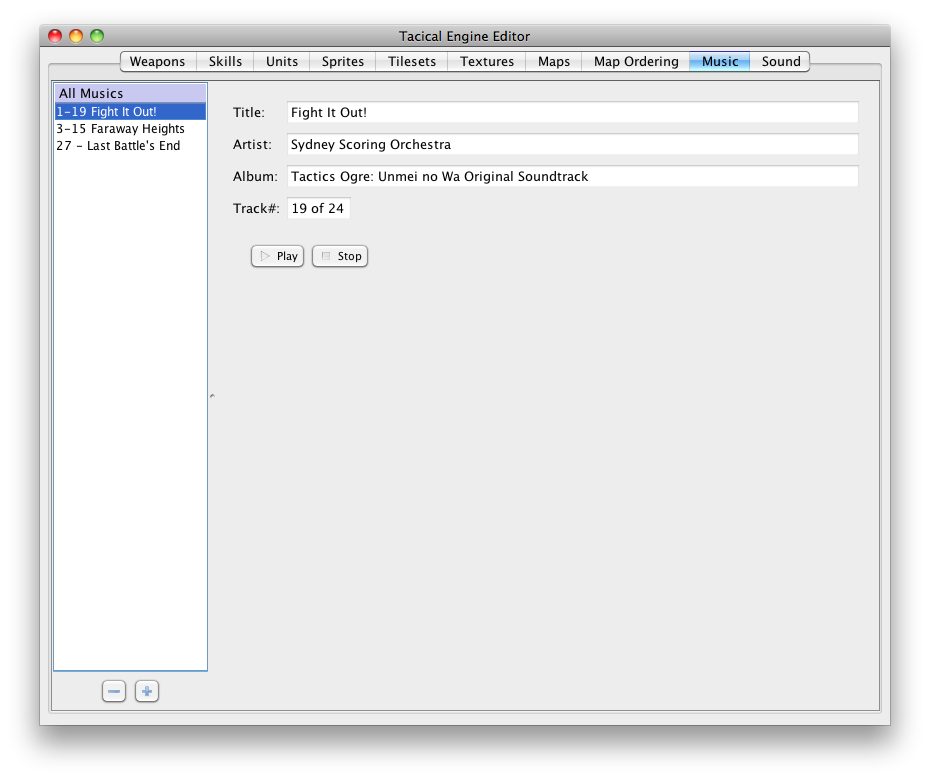
\includegraphics[width=0.75\textwidth]{figures/editor/Music.png}
	\caption{The Music Editor}
	\label{fig:figures_editor_Music}
\end{figure}
The music editor supports choosing which music is available to use in the game.  When a track is selected in the editor, the metadata (include the `artist' and `album') of the track is displayed.  As a further enhancement, the track can be previewed, this is especially useful when used in combination with the sound effect editor (which has exactly the same interface) to see what the combination of sounds and music sound like. 

\subsubsection{Map Editor}

\begin{figure}[htbp]
	\centering
		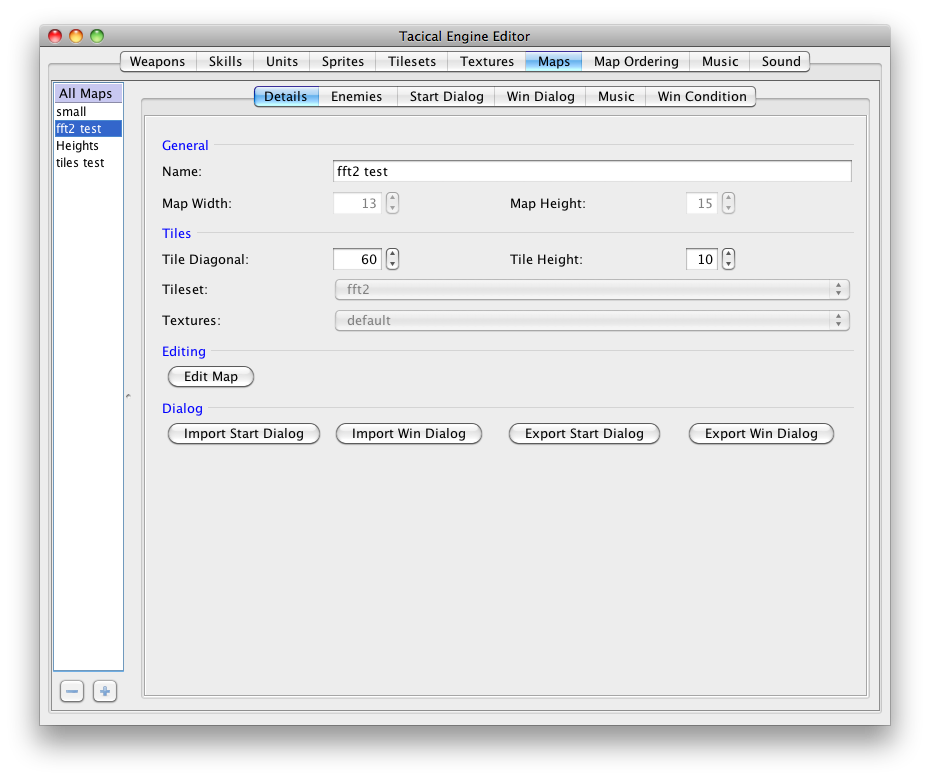
\includegraphics[width=.9\textwidth]{figures/editor/maps.png}
	\caption{The Map Editor}
	\label{fig:figures_editor_maps}
\end{figure}

The map allows the user to customise all of the aspects of a created map.  The editor is composed using a series of tabs so that the user does not get overwhelmed with all the options available. More importantly it allowed reuse of the unit editor(section \ref{ssub:unit_editors}) for enemy units (with the addition  of extra fields to allow customisation of the enemy behaviour).

Usually all the resources of an editor are loaded when the tab is selected and then cached.  While this did work for the maps, it caused unacceptable startup time hence I found an alternative method. 

\emph{Lazy Loading} only loads a resource when it is actually used instead of just been referenced\cite{Fowler:2002:PEA:579257}. In the case of the map editor a map is only loaded if the user tries to \emph{edit} the map. This significantly reduces loading time of the editor, especially if the user has created a large number of maps.

\paragraph{Details Tab\\}
The details tabs allows the user to change a map's name, as well as the size of the tiles.  The size of the map cannot be changed after creation to keep the implementation of the simple\footnote{Although the engine does support changing the map size.}. Another reason for not allowing the user to change the map size is that some of data, such as the enemy unit placement, may become invalid, which goes against the goal of always keeping the data consistent.  

For the same reasons, the editor does not let the user change the associated tileset or texture set after creating the map  although the engine does support it. Note that the user can still add tiles to the tileset, so it is not a large restriction.

The details tab also supports Dialog importing as well as exporting, which will be discussed in section \ref{ssub:dialog_editing}.

\paragraph{Music Tab\\}
The music tab allows the user to select from any music they imported into the music editor(section \ref{ssub:music_editor}).

\paragraph{Win Condition Tab\\}
This tab allows the user to choose the condition the player has to satisfy to win the map. Although the engine supports arbitrary conditions, the editor provides the two most common conditions used in TRPG, namely defeat all enemy units, and defeat a specific unit, which allows them  reasonable customisability.

\paragraph{Map Creation\\}
When creating the map, the user can specify the size of map and tileset to associate with the map.  An interesting addition to the editor is, as previously  mentioned, that it can use Stasyk's terrain generator which can be used as a starting point for the user's creations as shown in figure \ref{fig:figures_editor_gen}.

\begin{figure}[htb]
	\centering
		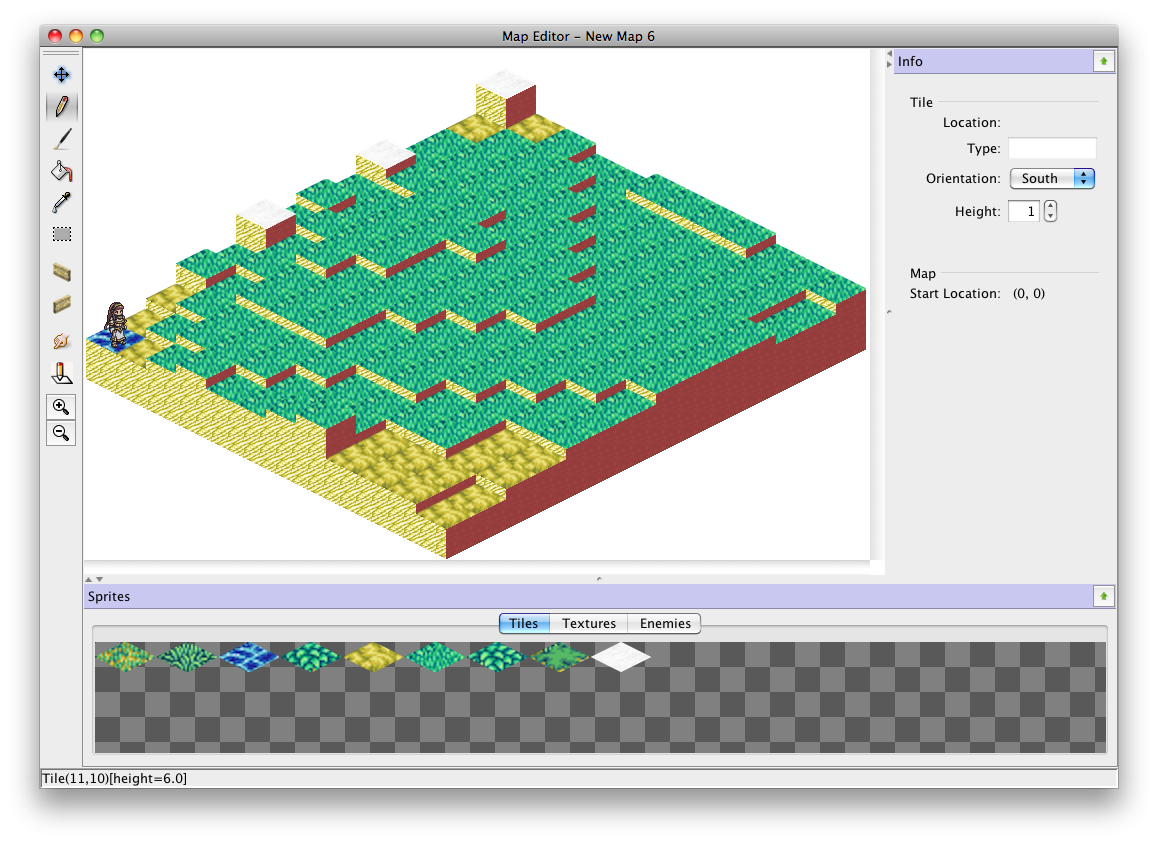
\includegraphics[width=\textwidth]{figures/editor/gen.png}
	\caption{The map editor shows a map created by Stasyk's terrain generator.}
	\label{fig:figures_editor_gen}
\end{figure}

\subsubsection{Visual Map Creation}
\label{ssub:visual_map_creation}

The visual map editor allows the user to design a map with writing any xml (the format the engine takes as input).  The editor shows the available tiles in the associated tileset in the bottom split.  The user can use the tools on the tool palette on the left to place the tiles.  The tools include:

\begin{description}
	\item[Move]   Allows the user to move the map.
	\item[Pencil] Draws the selected tile in \texttt{Tiles} on to any tile that is clicked on the map.
	\item[Brush]  Same as Pencil but sets the height and orientation as well (from the info panel).
	\item[Paint]  Sets the image of \emph{all} tiles in the selected area.
	\item[Eyedropper]  Sets the selected tile in \texttt{Tiles} to the image of the clicked tile.
	\item[Area Tool]  Used to select a number of tiles on the map.
	\item[Left Wall]  Sets the texture of the left wall.
	\item[Right Wall] Sets the texture of the right wall.
	\item[Pointing Finger]  Places enemy units on the map.
	\item[Pointer to Tile]  Sets the player's start location.
\end{description}

The panel on the right displays data on the selected tile on the map. It also allows the user to edit the orientation and height of the tile.  As shown in figure \ref{fig:figures_editor_Map}  tiles can be hidden. This allows more customisability, e.g. it could be used to make ``islands''  (a set of tiles with empty tiles around them),  and a set of bridges between them. 

The visual map editor supports editing  of both textured and non-textured tiles. As discussed before, non-textured tiles allow the user more control over what is drawn, so they  apply more detail. The advantage of textured tiles is that slanted tiles can be used, which easily allows the creation of slopes and stairs for example.


\clearpage
\subsubsection{Dialog Editing}
\label{ssub:dialog_editing}

\begin{figure}[htbp]
	\centering
		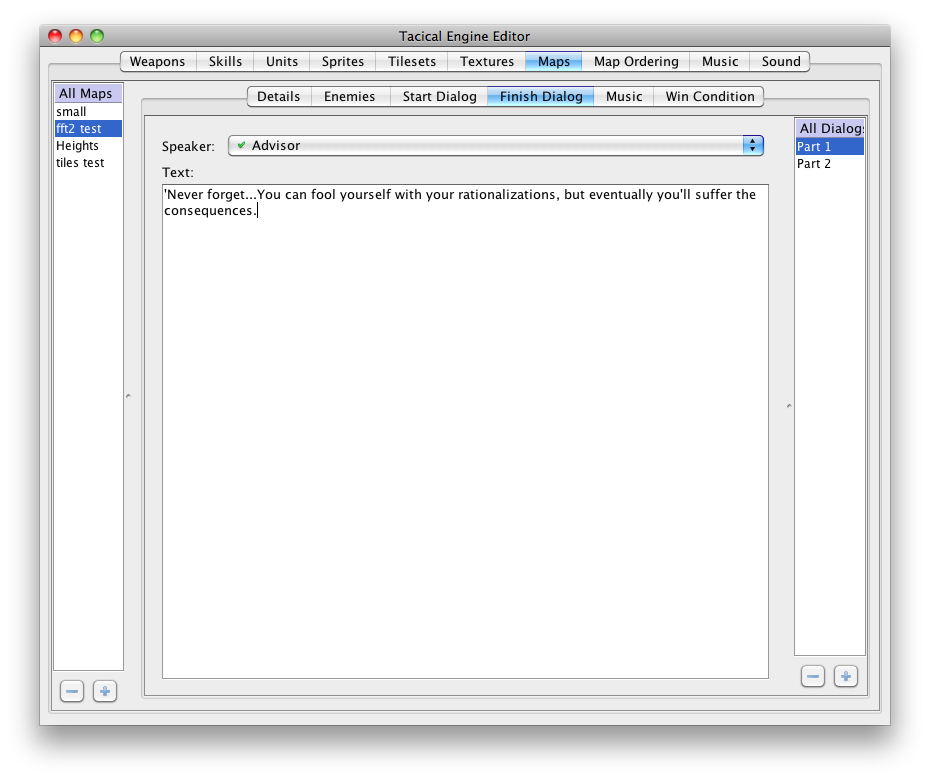
\includegraphics[height=4in]{figures/editor/Maps-dialog.png}
	\caption{The dialog editing panel}
	\label{fig:figures_editor_Maps-dialog}
\end{figure}
The editor supports the creation of dialog.  A dialog is a sequence of parts. Each part has the text  associated with it as well as optionally having a speaker.  The speaker can be selected from any unit that has already been placed on the map. This is a vast improvement on the original design where the user types the name of the speaker since there is no chance of entering invalid data.

As mentioned before, the engine takes care of pagination as well as line wrapping when displaying the dialog in the game. This frees the user from having to fit the text into a specified area. 

\paragraph{Import/Export\\}
The editor also supports importing as well as exporting the dialog in the format shown below. 
\begin{lstlisting}[caption=Shows the format used  for the dialog]
- speaker1: Some text 
- speaker2: Some more text
- none:     This part has no speaker
\end{lstlisting}
This allows the dialog to be easily written in the user's preferred application.  This could be useful if a  separate person writes the dialog of the game since the person does not need a copy of the editor. The format is described in more detail in the appendix \ref{ssub:dialog_data_format}  

Although the dialog xml format could be edited by the determined user, this would require significantly more effect then the above format since the user would have to find the unique id  of each unit each they want use as a speaker. It would also require creating unique ids for dialog part which would be likely be error prone, hence the above format is used in import/export, mainly for the user's convenience.

\subsubsection{Project Selection}
\begin{figure}[htbp]
	\centering
		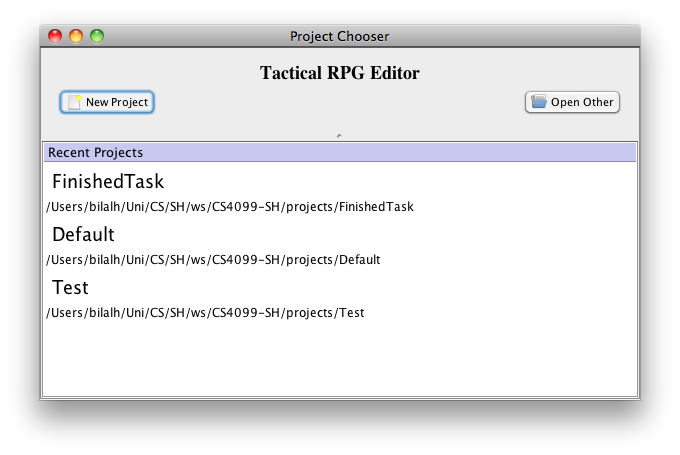
\includegraphics[width=1.05\textwidth]{figures/editor/Project_Selection.png}
	\caption{The project selection window which is shown at startup}
	\label{fig:figures_editor_Project_Selection}
\end{figure}

When the editor starts, it displays the above startup screen which allows the user to create a new project or open an existing project.  Since a user is likely to work on the same project for a significant period of time, the editor keeps tracks of recent projects. 

%TODO put bug when loading music stops
\subsubsection{Exporting}
\label{ssub:exporting}

The editor can export the game as a complete package, either as a Mac OS X application or as jar. These applications don't require any external resources, apart from a recent version of Java\footnote{specifically Java 1.6+}.

A prominent feature of the editor is that the jar will work on any Java enabled platform, since the jar contains all required libraries for each platform. The OS X application can even be exported on other platforms.

While most of the testing was done on OS X \footnote{Mac OS X 10.6 Snow leopard}, it also works well on Linux \footnote{Science  Linux x.y}. It  even has limited compatibly with Windows \footnote{Tested on Windows 7 32 bit} (apart from some minor graphics issues).

\subsection{Ant Build File}

The task of creating the Editor as a self contained application with no external dependencies, apart from obviously Java is non-trivial and error prone.  To automate this task, an Ant build file was created, which has an added benefit of allowing the creation of the distribution from the command line. 

The main steps to create the self contained editor are:
\begin{itemize}
	\item Compiling the code.
	\item Creating the jar of the engine.
	\item Creating the jar of the editor
	\item Creating the directory structure for the editor Mac OS X application.
	\begin{itemize}[topsep=0mm,noitemsep ]
		\item This includes creating the plist\cite{plist} with the applications.
		\item Setup the native libraries and the Java include path.
		\item Adds the icons.
		\item Link the Java wrapper so that the application can run, as well as having the  icons appears in the Dock.
	\end{itemize}
	\item Create the cross platform jar for the editor. 
	\begin{itemize}[topsep=0mm,noitemsep ]
		\item Combines the jars into a single jar.
		\item Set up the native libraries path.
		\item Set up the Java libraries path.
	\end{itemize}
	\item Create the cross platform jar for exporting the game.
	\item Create Mac OS X application for exporting the game.
	\item Copy the resources for the starting project.
\end{itemize}

The ant build file takes care of all the above steps and can be invoked by executing \lstinline{ant dist}. The build file has many other features such as running all tests and creating a web page. These features are described at the top of the build file (\texttt{build.xml}).

